\documentclass[11pt,a4paper]{article}

\usepackage[T1]{fontenc}
\usepackage[utf8]{inputenc}
\usepackage[british]{babel}
\usepackage[left=0mm,right=0mm,top=0mm,bottom=0mm]{geometry}
\usepackage[stretch=25,shrink=25,tracking=true,letterspace=30]{microtype}
\usepackage{graphicx}
\usepackage{xcolor}
\usepackage{marvosym}
\usepackage{enumitem}
\setlist{parsep=0pt,topsep=0pt,partopsep=1pt,itemsep=1pt,leftmargin=6mm}
\usepackage{FiraSans}
\renewcommand{\familydefault}{\sfdefault}
\definecolor{cvblue}{HTML}{304263}

% --- Macros perso ------------------------------------------------------------
\newcommand{\dates}[1]{\hfill\mbox{\textbf{#1}}}
\newcommand{\is}{\par\vskip.5ex plus .4ex}
\newcommand{\smaller}[1]{{\small$\diamond$\ #1}}
\newcommand{\headleft}[1]{\vspace*{3ex}\textsc{\textbf{#1}}\par%
    \vspace*{-1.5ex}\hrulefill\par\vspace*{0.7ex}}
\newcommand{\headright}[1]{\vspace*{2.5ex}\textsc{\Large\color{cvblue}#1}\par%
     \vspace*{-2ex}{\color{cvblue}\hrulefill}\par}

\usepackage[colorlinks=true,urlcolor=white,linkcolor=white]{hyperref}

% -----------------------------------------------------------------------------


\begin{document}
\setlength{\topskip}{0pt}\setlength{\parindent}{0pt}\setlength{\parskip}{0pt}
\setlength{\fboxsep}{0pt}\pagestyle{empty}\raggedbottom

% ============================================================================
%                               COLONNE GAUCHE
% ============================================================================
\begin{minipage}[t]{0.33\textwidth}
\colorbox{cvblue}{\begin{minipage}[t][5mm][t]{\textwidth}\null\hfill\null\end{minipage}}
\vspace{-.2ex}
\colorbox{cvblue!90}{\color{white}
\kern0.09\textwidth
\begin{minipage}[t][293mm][t]{0.82\textwidth}\raggedright
\vspace*{2.5ex}

% ---- Identité ---------------------------------------------------------------
\Large Pape Saliou \textbf{\textsc{FALL}} \normalsize

\null\hfill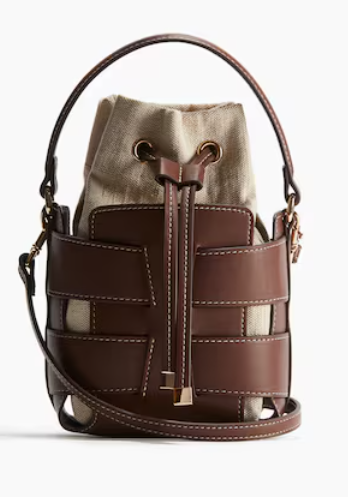
\includegraphics[width=0.65\textwidth]{ 70b0aeef46744dac9ceba7301f30bd8a.png }\hfill\null

\vspace*{0.5ex}

% ---- Résumé -----------------------------------------------------------------
\headleft{Profile Summary}
Data Scientist avec une solide formation académique (Master 2 en Data Science à la Sorbonne) et une expérience professionnelle significative dans la construction, le déploiement et l’optimisation de modèles prédictifs. Compétent en Python, SQL, Machine Learning, MLOps et visualisation de données, avec un intérêt marqué pour la résolution de problématiques métier à fort impact.

% ---- Contact ----------------------------------------------------------------
\headleft{Contact details}\small
\MVAt\ {\small papesalioufall2@gmail.com} \\[0.4ex]
\Mobilefone\ 0753481453 \\[0.5ex]
\Letter\ Paris, Île-de-France, France
\normalsize

% ---- Infos perso ------------------------------------------------------------
\headleft{Personal information}
Citizenship: \textbf{Française} \\[0.5ex]
Family: \textbf{Célibataire} \\[0.5ex]
Languages: \textbf{Français, Anglais}

% ---- Compétences ------------------------------------------------------------
\headleft{Skills}
\begin{itemize}
  \item Python
  \item SQL
  \item Machine Learning (scikit-learn, XGBoost, LightGBM)
  \item Deep Learning (TensorFlow, Keras)
  \item Data Visualisation (Matplotlib, Seaborn, Power BI)
  \item MLOps (MLflow, Docker, Git, CI/CD)
  \item Cloud Computing (AWS, Azure)
  \item Statistiques avancées
  \item Traitement du langage naturel (NLP)
\end{itemize}

\end{minipage}\kern 0.09\textwidth
}
\end{minipage}
% ============================================================================
%                               COLONNE DROITE
% ============================================================================
\hskip2.5em
\begin{minipage}[t]{0.56\textwidth}
\setlength{\parskip}{0.8ex}
\vspace{2ex}

% ------------------------ EXPÉRIENCE ----------------------------------------
\headright{Experience}
\textsc{data scientist} at \textit{Prepaya} (Paris, France)  \dates{2022-2024} \\
\smaller{Développé des modèles de scoring de crédit améliorant l’AUC de 15 \%.}\is
\smaller{Implémenté des pipelines de Machine Learning end-to-end en Python (scikit-learn, MLflow).}\is
\smaller{Déployé des modèles en production via Docker et AWS, réduisant le temps de mise en ligne de 30 \%.}\is
\smaller{Réalisé des analyses exploratoires et des dashboards Power BI pour orienter la stratégie produit.}\is
\smaller{Optimisé des requêtes SQL sur des bases de données volumineuses (>50 M lignes).}\is
\smaller{Collaboré avec les équipes produit, marketing et finance pour traduire les besoins métiers en solutions data.}\is

% ------------------------ ÉDUCATION ----------------------------------------
\headright{Education}
\textsc{Master 2 Data science}. \textit{Sorbonne Université}. \dates{2022-2023} \\

% ------------------------ CERTIFICATIONS ------------------------------------
\headright{Certifications}
\smaller{\textsc{DP-100 : Designing and Implementing a Data Science Solution on Azure}}, \textit{Microsoft}. \dates{2023-11} \\
\smaller{\textsc{AWS Certified Machine Learning – Specialty}}, \textit{Amazon Web Services}. \dates{2024-05} \\

% ------------------------ HOBBIES -------------------------------------------
\headright{Hobbies}
\textit{Course à pied, lecture de science-fiction, photographie urbaine}

\end{minipage}

\end{document}